\begin{figure}
\centering
\begin{subfigure}{0.55\textwidth}
    \begin{center}
        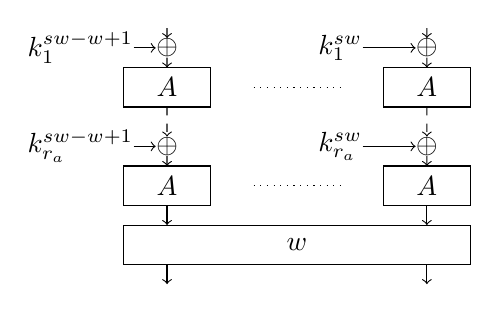
\begin{tikzpicture}[xscale=1.1, yscale=0.5]
            \draw (+0.0, 0.0) rectangle node[pos=0.5]{$\linLayer{w}$} (+4.0, 1.0) ;
            \draw[->] (+0.5, 0.0) -- (+0.5, -0.5) ;
            \draw[->] (+3.5, 0.0) -- (+3.5, -0.5) ;
            % First column
            \draw (+0.5, 5.5) node[inner sep=0](xor01){$\oplus$};
            \draw[->] (+0.5, 6.0) -- (xor01) ;
            \draw[->] (xor01) -- (+0.5, 5.0);
            \draw (+0.0, 4.0) rectangle node[pos=0.5]{$A$} (+1.0, 5.0) ;
            \draw (+0.0, 1.5) rectangle node[pos=0.5]{$A$} (+1.0, 2.5) ;
            \draw (+0.5, 3.0) node[inner sep=0](xor00){$\oplus$};
            \draw[dashed,->] (+0.5, 4.0) -- (xor00) ;
`            \draw[->] (xor00) -- (+0.5, 2.5) ;
            \draw[->] (+0.5, 1.5) -- (+0.5, 1.0) ;
            % Second column
            \draw (+3.5, 5.5) node[inner sep=0](xor11){$\oplus$};
            \draw[->] (+3.5, 6.0) -- (xor11) ;
            \draw[->] (xor11) -- (+3.5, 5.0);
            \draw (+3.0, 4.0) rectangle node[pos=0.5]{$A$} (+4.0, 5.0) ;
            \draw (+3.0, 1.5) rectangle node[pos=0.5]{$A$} (+4.0, 2.5) ;
            \draw (+3.5, 3.0) node[inner sep=0](xor10){$\oplus$};
            \draw[dashed,->] (+3.5, 4.0) -- (xor10) ;
            \draw[->] (xor10) -- (+3.5, 2.5) ;
            \draw[->] (+3.5, 1.5) -- (+3.5, 1.0) ;
            % key addition
            \draw (-0.5, 5.5) node[inner sep=0](k_top_left){$k^{sw-w+1}_1$} ;
            \draw[->] (k_top_left) -- (xor01) ;
            \draw (-0.5, 3.0) node[inner sep=0](k_bottom_left){$k^{sw-w+1}_{r_a}$} ;
            \draw[->] (k_bottom_left) -- (xor00) ;
            \draw (+2.5, 5.5) node[inner sep=0](k_top_right){$k^{sw}_1$} ;
            \draw[->] (k_top_right) -- (xor11) ;
            \draw (+2.5, 3.0) node[inner sep=0](k_bottom_right){$k^{sw}_{r_a}$} ;
            \draw[->] (k_bottom_right) -- (xor10) ;
            % ellipses
            \draw[dotted] (+1.5, +4.5) -- (+2.5, +4.5) ;
            \draw[dotted] (+1.5, +2.0) -- (+2.5, +2.0) ;
        \end{tikzpicture}
        \caption{A step of \sparx{}.}
    \end{center}
\end{subfigure}
\hspace{2em}
\begin{subfigure}{0.35\textwidth}
    \begin{center}
        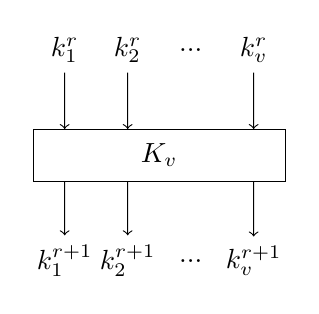
\begin{tikzpicture}[xscale=0.8, yscale=0.67]
            % input
            \draw (+0.5, +5.0) node(k00){$k^{r}_1$} ;
            \draw (+1.5, +5.0) node(k01){$k^{r}_2$} ;
            \draw (+2.5, +5.0) node{...} ;
            \draw (+3.5, +5.0) node(k0f){$k^{r}_{v}$} ;
            % permutation
            \draw (+0.0, +2.5) rectangle node[pos=0.5]{$K_v$} (+4.0, +3.5) ;
            % output
            \draw (+0.5, +1.0) node(k10){$k^{r+1}_1$} ;
            \draw (+1.5, +1.0) node(k11){$k^{r+1}_2$} ;
            \draw (+2.5, +1.0) node{...} ;
            \draw (+3.5, +1.0) node(k1f){$k^{r+1}_{v}$} ;
            % Arrows
            \draw[->] (k00) -- (+0.5, +3.5) ;
            \draw[->] (k01) -- (+1.5, +3.5) ;
            \draw[->] (k0f) -- (+3.5, +3.5) ;
            \draw[->] (+0.5, +2.5) -- (k10) ;
            \draw[->] (+1.5, +2.5) -- (k11) ;
            \draw[->] (+3.5, +2.5) -- (k1f) ;
        \end{tikzpicture}
        \caption{Key schedule.}
    \end{center}
\end{subfigure}
% \begin{subfigure}{0.25\textwidth}
%     \begin{center}
%         \begin{tikzpicture}[scale=0.5]
%             % operations
%             % \draw (-2.9, +4.6) rectangle node[pos=0.5]{$\oplus k^i_r$} (+2.9, +5.6) ;
%             \draw (-3.0, +3.5) rectangle node[pos=0.5]{$\ggg 7$} (-1.0, +4.5) ;
%             \draw (-2.0, +2.5) node[inner sep=0](add){$\boxplus$} ;
%             \draw (+1.0, +1.0) rectangle node[pos=0.5]{$\lll 2$} (+3.0, +2.0) ;
%             \draw (+2.0, +0.0) node[inner sep=0](xor){$\oplus$} ;
%             % arrows
%             \draw[->] (-2.0, +5.0) -- (-2.0, +4.5) ;
%             \draw[->] (+2.0, +5.0) -- (+2.0, +2.0) ;
%             \draw[->] (-2.0, +3.5) -- (add) ;
%             \draw[->] (+2.0, +2.5) -- (add) ;
%             \draw[->] (add) -- (-2.0, -1.0) ;
%             \draw[->] (+2.0, +1.0) -- (xor) ;
%             \draw[->] (-2.0, +0.0) -- (xor) ;
%             \draw[->] (xor) -- (+2.0, -1.0) ;
%         \end{tikzpicture}
%         \FigDef{speckey}{$A$}
%     \end{center}
% \end{subfigure}
\FigDef{sparx}{A high-level view of a step $s$ of \sparx{}}
\end{figure}